\documentclass[10pt,twocolumn]{article}
\usepackage{graphicx}
\usepackage[margin=0.5in]{geometry}
\usepackage[cmex10]{amsmath}
\usepackage{array}
\usepackage{booktabs}
\usepackage{mathtools}
\title{\textbf{Optimization Assignment - 1}}
\author{GANGA GOPINATH}



\providecommand{\norm}[1]{\left\lVert#1\right\rVert}
\providecommand{\abs}[1]{\left\vert#1\right\vert}
\let\vec\mathbf
\newcommand{\myvec}[1]{\ensuremath{\begin{pmatrix}#1\end{pmatrix}}}
\newcommand{\mydet}[1]{\ensuremath{\begin{vmatrix}#1\end{vmatrix}}}
\providecommand{\brak}[1]{\ensuremath{\left(#1\right)}}
\providecommand{\lbrak}[1]{\ensuremath{\left(#1\right.}}
\providecommand{\rbrak}[1]{\ensuremath{\left.#1\right)}}
\providecommand{\sbrak}[1]{\ensuremath{{}\left[#1\right]}}

\begin{document}

\maketitle
\paragraph{\textit{Problem Statement} - A manufacturer produces two types of steel trunks. He has two machines A and
B. The first type of the trunk requires 3 hours on machine A and 3 hours on machine B. The second type of trunk requires 3 hours on machine A and 2 hours on machine B. Machines A and B are run daily for 18 hours and 15 hours respectively. There is a profit of Rs. 30 on the first type of the trunk and Rs. 25 on the second type of the trunk. How many trunks of each type
should be produced and sold to make maximum profit ?} 

\section*{\large Solution}
Let x,y be the trunk of first type $\&$ second type were manufactured respectively.
\begin{center}
    \setlength{\arrayrulewidth}{0.1mm}
	\setlength{\tabcolsep}{2pt}
	\renewcommand{\arraystretch}{2}
\begin{tabular}{|c|c|c|c|}
	\hline 
    \textbf{} & \textbf{Machine A (hrs)} & \textbf{Machine B (hrs)} \\ \hline
    First type(x) & 3 &  3 \\ \hline
    Second type(y) & 3 & 3\\ \hline
     Availability & 18 & 15\\ \hline
\end{tabular}\\ \vspace{2mm}
\hspace{1cm} Table 1
\end{center}
Therefore, the constraints are
\begin{align}
3x + 3y \leq 18 \\
3x + 2y \leq 15
\end{align}
Profit of Rs 30 and Rs 25 per trunk of the first type and the second type respectively. Let P be the maximum profit from x trunks of first type and y trunks of second type is Rs 30x and Rs 25y respectively.The problem can be formulated as
\begin{align}
	P = \max_{x,y}(30x+25y)
\end{align}
which can be expressed in vector form as
\begin{align}
	P = \max_{\vec{x}}\myvec{30&25}\vec{x}\\
	\myvec{3 & 3 \\ 3 & 2 \\ 1 & 0\\0&1}\vec{x} \leq \myvec{18 \\ 15\\0\\0}\\
	\vec{x} \geq \vec{0}
\end{align}
Solving the above equations using cvxpy, we get
\begin{align}
	P_{max} = 165\\
	\vec{x} = \myvec{3 \\ 3}
\end{align}
\begin{center}
 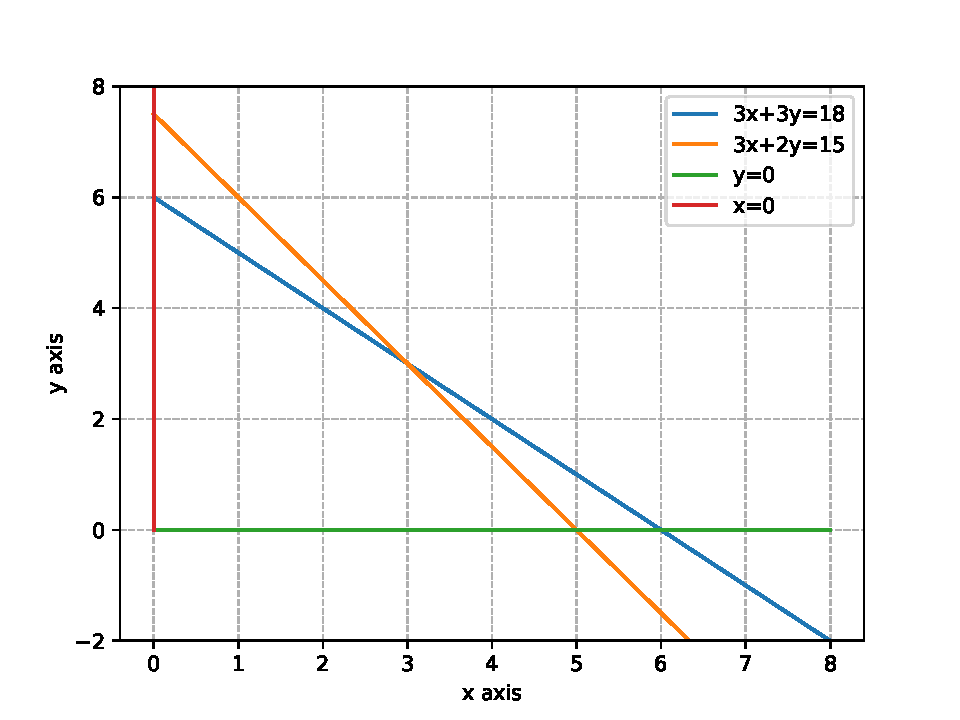
\includegraphics[width=0.5\textwidth]{opt1.pdf}  
 \end{center}\vspace{1mm}
\end{document}